
% Default to the notebook output style

    


% Inherit from the specified cell style.




    
\documentclass[11pt]{article}

    
    
    \usepackage[T1]{fontenc}
    % Nicer default font (+ math font) than Computer Modern for most use cases
    \usepackage{mathpazo}

    % Basic figure setup, for now with no caption control since it's done
    % automatically by Pandoc (which extracts ![](path) syntax from Markdown).
    \usepackage{graphicx}
    % We will generate all images so they have a width \maxwidth. This means
    % that they will get their normal width if they fit onto the page, but
    % are scaled down if they would overflow the margins.
    \makeatletter
    \def\maxwidth{\ifdim\Gin@nat@width>\linewidth\linewidth
    \else\Gin@nat@width\fi}
    \makeatother
    \let\Oldincludegraphics\includegraphics
    % Set max figure width to be 80% of text width, for now hardcoded.
    \renewcommand{\includegraphics}[1]{\Oldincludegraphics[width=.8\maxwidth]{#1}}
    % Ensure that by default, figures have no caption (until we provide a
    % proper Figure object with a Caption API and a way to capture that
    % in the conversion process - todo).
    \usepackage{caption}
    \DeclareCaptionLabelFormat{nolabel}{}
    \captionsetup{labelformat=nolabel}

    \usepackage{adjustbox} % Used to constrain images to a maximum size 
    \usepackage{xcolor} % Allow colors to be defined
    \usepackage{enumerate} % Needed for markdown enumerations to work
    \usepackage{geometry} % Used to adjust the document margins
    \usepackage{amsmath} % Equations
    \usepackage{amssymb} % Equations
    \usepackage{textcomp} % defines textquotesingle
    % Hack from http://tex.stackexchange.com/a/47451/13684:
    \AtBeginDocument{%
        \def\PYZsq{\textquotesingle}% Upright quotes in Pygmentized code
    }
    \usepackage{upquote} % Upright quotes for verbatim code
    \usepackage{eurosym} % defines \euro
    \usepackage[mathletters]{ucs} % Extended unicode (utf-8) support
    \usepackage[utf8x]{inputenc} % Allow utf-8 characters in the tex document
    \usepackage{fancyvrb} % verbatim replacement that allows latex
    \usepackage{grffile} % extends the file name processing of package graphics 
                         % to support a larger range 
    % The hyperref package gives us a pdf with properly built
    % internal navigation ('pdf bookmarks' for the table of contents,
    % internal cross-reference links, web links for URLs, etc.)
    \usepackage{hyperref}
    \usepackage{longtable} % longtable support required by pandoc >1.10
    \usepackage{booktabs}  % table support for pandoc > 1.12.2
    \usepackage[inline]{enumitem} % IRkernel/repr support (it uses the enumerate* environment)
    \usepackage[normalem]{ulem} % ulem is needed to support strikethroughs (\sout)
                                % normalem makes italics be italics, not underlines
    

    
    
    % Colors for the hyperref package
    \definecolor{urlcolor}{rgb}{0,.145,.698}
    \definecolor{linkcolor}{rgb}{.71,0.21,0.01}
    \definecolor{citecolor}{rgb}{.12,.54,.11}

    % ANSI colors
    \definecolor{ansi-black}{HTML}{3E424D}
    \definecolor{ansi-black-intense}{HTML}{282C36}
    \definecolor{ansi-red}{HTML}{E75C58}
    \definecolor{ansi-red-intense}{HTML}{B22B31}
    \definecolor{ansi-green}{HTML}{00A250}
    \definecolor{ansi-green-intense}{HTML}{007427}
    \definecolor{ansi-yellow}{HTML}{DDB62B}
    \definecolor{ansi-yellow-intense}{HTML}{B27D12}
    \definecolor{ansi-blue}{HTML}{208FFB}
    \definecolor{ansi-blue-intense}{HTML}{0065CA}
    \definecolor{ansi-magenta}{HTML}{D160C4}
    \definecolor{ansi-magenta-intense}{HTML}{A03196}
    \definecolor{ansi-cyan}{HTML}{60C6C8}
    \definecolor{ansi-cyan-intense}{HTML}{258F8F}
    \definecolor{ansi-white}{HTML}{C5C1B4}
    \definecolor{ansi-white-intense}{HTML}{A1A6B2}

    % commands and environments needed by pandoc snippets
    % extracted from the output of `pandoc -s`
    \providecommand{\tightlist}{%
      \setlength{\itemsep}{0pt}\setlength{\parskip}{0pt}}
    \DefineVerbatimEnvironment{Highlighting}{Verbatim}{commandchars=\\\{\}}
    % Add ',fontsize=\small' for more characters per line
    \newenvironment{Shaded}{}{}
    \newcommand{\KeywordTok}[1]{\textcolor[rgb]{0.00,0.44,0.13}{\textbf{{#1}}}}
    \newcommand{\DataTypeTok}[1]{\textcolor[rgb]{0.56,0.13,0.00}{{#1}}}
    \newcommand{\DecValTok}[1]{\textcolor[rgb]{0.25,0.63,0.44}{{#1}}}
    \newcommand{\BaseNTok}[1]{\textcolor[rgb]{0.25,0.63,0.44}{{#1}}}
    \newcommand{\FloatTok}[1]{\textcolor[rgb]{0.25,0.63,0.44}{{#1}}}
    \newcommand{\CharTok}[1]{\textcolor[rgb]{0.25,0.44,0.63}{{#1}}}
    \newcommand{\StringTok}[1]{\textcolor[rgb]{0.25,0.44,0.63}{{#1}}}
    \newcommand{\CommentTok}[1]{\textcolor[rgb]{0.38,0.63,0.69}{\textit{{#1}}}}
    \newcommand{\OtherTok}[1]{\textcolor[rgb]{0.00,0.44,0.13}{{#1}}}
    \newcommand{\AlertTok}[1]{\textcolor[rgb]{1.00,0.00,0.00}{\textbf{{#1}}}}
    \newcommand{\FunctionTok}[1]{\textcolor[rgb]{0.02,0.16,0.49}{{#1}}}
    \newcommand{\RegionMarkerTok}[1]{{#1}}
    \newcommand{\ErrorTok}[1]{\textcolor[rgb]{1.00,0.00,0.00}{\textbf{{#1}}}}
    \newcommand{\NormalTok}[1]{{#1}}
    
    % Additional commands for more recent versions of Pandoc
    \newcommand{\ConstantTok}[1]{\textcolor[rgb]{0.53,0.00,0.00}{{#1}}}
    \newcommand{\SpecialCharTok}[1]{\textcolor[rgb]{0.25,0.44,0.63}{{#1}}}
    \newcommand{\VerbatimStringTok}[1]{\textcolor[rgb]{0.25,0.44,0.63}{{#1}}}
    \newcommand{\SpecialStringTok}[1]{\textcolor[rgb]{0.73,0.40,0.53}{{#1}}}
    \newcommand{\ImportTok}[1]{{#1}}
    \newcommand{\DocumentationTok}[1]{\textcolor[rgb]{0.73,0.13,0.13}{\textit{{#1}}}}
    \newcommand{\AnnotationTok}[1]{\textcolor[rgb]{0.38,0.63,0.69}{\textbf{\textit{{#1}}}}}
    \newcommand{\CommentVarTok}[1]{\textcolor[rgb]{0.38,0.63,0.69}{\textbf{\textit{{#1}}}}}
    \newcommand{\VariableTok}[1]{\textcolor[rgb]{0.10,0.09,0.49}{{#1}}}
    \newcommand{\ControlFlowTok}[1]{\textcolor[rgb]{0.00,0.44,0.13}{\textbf{{#1}}}}
    \newcommand{\OperatorTok}[1]{\textcolor[rgb]{0.40,0.40,0.40}{{#1}}}
    \newcommand{\BuiltInTok}[1]{{#1}}
    \newcommand{\ExtensionTok}[1]{{#1}}
    \newcommand{\PreprocessorTok}[1]{\textcolor[rgb]{0.74,0.48,0.00}{{#1}}}
    \newcommand{\AttributeTok}[1]{\textcolor[rgb]{0.49,0.56,0.16}{{#1}}}
    \newcommand{\InformationTok}[1]{\textcolor[rgb]{0.38,0.63,0.69}{\textbf{\textit{{#1}}}}}
    \newcommand{\WarningTok}[1]{\textcolor[rgb]{0.38,0.63,0.69}{\textbf{\textit{{#1}}}}}
    
    
    % Define a nice break command that doesn't care if a line doesn't already
    % exist.
    \def\br{\hspace*{\fill} \\* }
    % Math Jax compatability definitions
    \def\gt{>}
    \def\lt{<}
    % Document parameters
    \title{Tutorial-3-Dealing\_with\_complicated\_implication\_networks}
    
    
    

    % Pygments definitions
    
\makeatletter
\def\PY@reset{\let\PY@it=\relax \let\PY@bf=\relax%
    \let\PY@ul=\relax \let\PY@tc=\relax%
    \let\PY@bc=\relax \let\PY@ff=\relax}
\def\PY@tok#1{\csname PY@tok@#1\endcsname}
\def\PY@toks#1+{\ifx\relax#1\empty\else%
    \PY@tok{#1}\expandafter\PY@toks\fi}
\def\PY@do#1{\PY@bc{\PY@tc{\PY@ul{%
    \PY@it{\PY@bf{\PY@ff{#1}}}}}}}
\def\PY#1#2{\PY@reset\PY@toks#1+\relax+\PY@do{#2}}

\expandafter\def\csname PY@tok@w\endcsname{\def\PY@tc##1{\textcolor[rgb]{0.73,0.73,0.73}{##1}}}
\expandafter\def\csname PY@tok@c\endcsname{\let\PY@it=\textit\def\PY@tc##1{\textcolor[rgb]{0.25,0.50,0.50}{##1}}}
\expandafter\def\csname PY@tok@cp\endcsname{\def\PY@tc##1{\textcolor[rgb]{0.74,0.48,0.00}{##1}}}
\expandafter\def\csname PY@tok@k\endcsname{\let\PY@bf=\textbf\def\PY@tc##1{\textcolor[rgb]{0.00,0.50,0.00}{##1}}}
\expandafter\def\csname PY@tok@kp\endcsname{\def\PY@tc##1{\textcolor[rgb]{0.00,0.50,0.00}{##1}}}
\expandafter\def\csname PY@tok@kt\endcsname{\def\PY@tc##1{\textcolor[rgb]{0.69,0.00,0.25}{##1}}}
\expandafter\def\csname PY@tok@o\endcsname{\def\PY@tc##1{\textcolor[rgb]{0.40,0.40,0.40}{##1}}}
\expandafter\def\csname PY@tok@ow\endcsname{\let\PY@bf=\textbf\def\PY@tc##1{\textcolor[rgb]{0.67,0.13,1.00}{##1}}}
\expandafter\def\csname PY@tok@nb\endcsname{\def\PY@tc##1{\textcolor[rgb]{0.00,0.50,0.00}{##1}}}
\expandafter\def\csname PY@tok@nf\endcsname{\def\PY@tc##1{\textcolor[rgb]{0.00,0.00,1.00}{##1}}}
\expandafter\def\csname PY@tok@nc\endcsname{\let\PY@bf=\textbf\def\PY@tc##1{\textcolor[rgb]{0.00,0.00,1.00}{##1}}}
\expandafter\def\csname PY@tok@nn\endcsname{\let\PY@bf=\textbf\def\PY@tc##1{\textcolor[rgb]{0.00,0.00,1.00}{##1}}}
\expandafter\def\csname PY@tok@ne\endcsname{\let\PY@bf=\textbf\def\PY@tc##1{\textcolor[rgb]{0.82,0.25,0.23}{##1}}}
\expandafter\def\csname PY@tok@nv\endcsname{\def\PY@tc##1{\textcolor[rgb]{0.10,0.09,0.49}{##1}}}
\expandafter\def\csname PY@tok@no\endcsname{\def\PY@tc##1{\textcolor[rgb]{0.53,0.00,0.00}{##1}}}
\expandafter\def\csname PY@tok@nl\endcsname{\def\PY@tc##1{\textcolor[rgb]{0.63,0.63,0.00}{##1}}}
\expandafter\def\csname PY@tok@ni\endcsname{\let\PY@bf=\textbf\def\PY@tc##1{\textcolor[rgb]{0.60,0.60,0.60}{##1}}}
\expandafter\def\csname PY@tok@na\endcsname{\def\PY@tc##1{\textcolor[rgb]{0.49,0.56,0.16}{##1}}}
\expandafter\def\csname PY@tok@nt\endcsname{\let\PY@bf=\textbf\def\PY@tc##1{\textcolor[rgb]{0.00,0.50,0.00}{##1}}}
\expandafter\def\csname PY@tok@nd\endcsname{\def\PY@tc##1{\textcolor[rgb]{0.67,0.13,1.00}{##1}}}
\expandafter\def\csname PY@tok@s\endcsname{\def\PY@tc##1{\textcolor[rgb]{0.73,0.13,0.13}{##1}}}
\expandafter\def\csname PY@tok@sd\endcsname{\let\PY@it=\textit\def\PY@tc##1{\textcolor[rgb]{0.73,0.13,0.13}{##1}}}
\expandafter\def\csname PY@tok@si\endcsname{\let\PY@bf=\textbf\def\PY@tc##1{\textcolor[rgb]{0.73,0.40,0.53}{##1}}}
\expandafter\def\csname PY@tok@se\endcsname{\let\PY@bf=\textbf\def\PY@tc##1{\textcolor[rgb]{0.73,0.40,0.13}{##1}}}
\expandafter\def\csname PY@tok@sr\endcsname{\def\PY@tc##1{\textcolor[rgb]{0.73,0.40,0.53}{##1}}}
\expandafter\def\csname PY@tok@ss\endcsname{\def\PY@tc##1{\textcolor[rgb]{0.10,0.09,0.49}{##1}}}
\expandafter\def\csname PY@tok@sx\endcsname{\def\PY@tc##1{\textcolor[rgb]{0.00,0.50,0.00}{##1}}}
\expandafter\def\csname PY@tok@m\endcsname{\def\PY@tc##1{\textcolor[rgb]{0.40,0.40,0.40}{##1}}}
\expandafter\def\csname PY@tok@gh\endcsname{\let\PY@bf=\textbf\def\PY@tc##1{\textcolor[rgb]{0.00,0.00,0.50}{##1}}}
\expandafter\def\csname PY@tok@gu\endcsname{\let\PY@bf=\textbf\def\PY@tc##1{\textcolor[rgb]{0.50,0.00,0.50}{##1}}}
\expandafter\def\csname PY@tok@gd\endcsname{\def\PY@tc##1{\textcolor[rgb]{0.63,0.00,0.00}{##1}}}
\expandafter\def\csname PY@tok@gi\endcsname{\def\PY@tc##1{\textcolor[rgb]{0.00,0.63,0.00}{##1}}}
\expandafter\def\csname PY@tok@gr\endcsname{\def\PY@tc##1{\textcolor[rgb]{1.00,0.00,0.00}{##1}}}
\expandafter\def\csname PY@tok@ge\endcsname{\let\PY@it=\textit}
\expandafter\def\csname PY@tok@gs\endcsname{\let\PY@bf=\textbf}
\expandafter\def\csname PY@tok@gp\endcsname{\let\PY@bf=\textbf\def\PY@tc##1{\textcolor[rgb]{0.00,0.00,0.50}{##1}}}
\expandafter\def\csname PY@tok@go\endcsname{\def\PY@tc##1{\textcolor[rgb]{0.53,0.53,0.53}{##1}}}
\expandafter\def\csname PY@tok@gt\endcsname{\def\PY@tc##1{\textcolor[rgb]{0.00,0.27,0.87}{##1}}}
\expandafter\def\csname PY@tok@err\endcsname{\def\PY@bc##1{\setlength{\fboxsep}{0pt}\fcolorbox[rgb]{1.00,0.00,0.00}{1,1,1}{\strut ##1}}}
\expandafter\def\csname PY@tok@kc\endcsname{\let\PY@bf=\textbf\def\PY@tc##1{\textcolor[rgb]{0.00,0.50,0.00}{##1}}}
\expandafter\def\csname PY@tok@kd\endcsname{\let\PY@bf=\textbf\def\PY@tc##1{\textcolor[rgb]{0.00,0.50,0.00}{##1}}}
\expandafter\def\csname PY@tok@kn\endcsname{\let\PY@bf=\textbf\def\PY@tc##1{\textcolor[rgb]{0.00,0.50,0.00}{##1}}}
\expandafter\def\csname PY@tok@kr\endcsname{\let\PY@bf=\textbf\def\PY@tc##1{\textcolor[rgb]{0.00,0.50,0.00}{##1}}}
\expandafter\def\csname PY@tok@bp\endcsname{\def\PY@tc##1{\textcolor[rgb]{0.00,0.50,0.00}{##1}}}
\expandafter\def\csname PY@tok@fm\endcsname{\def\PY@tc##1{\textcolor[rgb]{0.00,0.00,1.00}{##1}}}
\expandafter\def\csname PY@tok@vc\endcsname{\def\PY@tc##1{\textcolor[rgb]{0.10,0.09,0.49}{##1}}}
\expandafter\def\csname PY@tok@vg\endcsname{\def\PY@tc##1{\textcolor[rgb]{0.10,0.09,0.49}{##1}}}
\expandafter\def\csname PY@tok@vi\endcsname{\def\PY@tc##1{\textcolor[rgb]{0.10,0.09,0.49}{##1}}}
\expandafter\def\csname PY@tok@vm\endcsname{\def\PY@tc##1{\textcolor[rgb]{0.10,0.09,0.49}{##1}}}
\expandafter\def\csname PY@tok@sa\endcsname{\def\PY@tc##1{\textcolor[rgb]{0.73,0.13,0.13}{##1}}}
\expandafter\def\csname PY@tok@sb\endcsname{\def\PY@tc##1{\textcolor[rgb]{0.73,0.13,0.13}{##1}}}
\expandafter\def\csname PY@tok@sc\endcsname{\def\PY@tc##1{\textcolor[rgb]{0.73,0.13,0.13}{##1}}}
\expandafter\def\csname PY@tok@dl\endcsname{\def\PY@tc##1{\textcolor[rgb]{0.73,0.13,0.13}{##1}}}
\expandafter\def\csname PY@tok@s2\endcsname{\def\PY@tc##1{\textcolor[rgb]{0.73,0.13,0.13}{##1}}}
\expandafter\def\csname PY@tok@sh\endcsname{\def\PY@tc##1{\textcolor[rgb]{0.73,0.13,0.13}{##1}}}
\expandafter\def\csname PY@tok@s1\endcsname{\def\PY@tc##1{\textcolor[rgb]{0.73,0.13,0.13}{##1}}}
\expandafter\def\csname PY@tok@mb\endcsname{\def\PY@tc##1{\textcolor[rgb]{0.40,0.40,0.40}{##1}}}
\expandafter\def\csname PY@tok@mf\endcsname{\def\PY@tc##1{\textcolor[rgb]{0.40,0.40,0.40}{##1}}}
\expandafter\def\csname PY@tok@mh\endcsname{\def\PY@tc##1{\textcolor[rgb]{0.40,0.40,0.40}{##1}}}
\expandafter\def\csname PY@tok@mi\endcsname{\def\PY@tc##1{\textcolor[rgb]{0.40,0.40,0.40}{##1}}}
\expandafter\def\csname PY@tok@il\endcsname{\def\PY@tc##1{\textcolor[rgb]{0.40,0.40,0.40}{##1}}}
\expandafter\def\csname PY@tok@mo\endcsname{\def\PY@tc##1{\textcolor[rgb]{0.40,0.40,0.40}{##1}}}
\expandafter\def\csname PY@tok@ch\endcsname{\let\PY@it=\textit\def\PY@tc##1{\textcolor[rgb]{0.25,0.50,0.50}{##1}}}
\expandafter\def\csname PY@tok@cm\endcsname{\let\PY@it=\textit\def\PY@tc##1{\textcolor[rgb]{0.25,0.50,0.50}{##1}}}
\expandafter\def\csname PY@tok@cpf\endcsname{\let\PY@it=\textit\def\PY@tc##1{\textcolor[rgb]{0.25,0.50,0.50}{##1}}}
\expandafter\def\csname PY@tok@c1\endcsname{\let\PY@it=\textit\def\PY@tc##1{\textcolor[rgb]{0.25,0.50,0.50}{##1}}}
\expandafter\def\csname PY@tok@cs\endcsname{\let\PY@it=\textit\def\PY@tc##1{\textcolor[rgb]{0.25,0.50,0.50}{##1}}}

\def\PYZbs{\char`\\}
\def\PYZus{\char`\_}
\def\PYZob{\char`\{}
\def\PYZcb{\char`\}}
\def\PYZca{\char`\^}
\def\PYZam{\char`\&}
\def\PYZlt{\char`\<}
\def\PYZgt{\char`\>}
\def\PYZsh{\char`\#}
\def\PYZpc{\char`\%}
\def\PYZdl{\char`\$}
\def\PYZhy{\char`\-}
\def\PYZsq{\char`\'}
\def\PYZdq{\char`\"}
\def\PYZti{\char`\~}
% for compatibility with earlier versions
\def\PYZat{@}
\def\PYZlb{[}
\def\PYZrb{]}
\makeatother


    % Exact colors from NB
    \definecolor{incolor}{rgb}{0.0, 0.0, 0.5}
    \definecolor{outcolor}{rgb}{0.545, 0.0, 0.0}



    
    % Prevent overflowing lines due to hard-to-break entities
    \sloppy 
    % Setup hyperref package
    \hypersetup{
      breaklinks=true,  % so long urls are correctly broken across lines
      colorlinks=true,
      urlcolor=urlcolor,
      linkcolor=linkcolor,
      citecolor=citecolor,
      }
    % Slightly bigger margins than the latex defaults
    
    \geometry{verbose,tmargin=1in,bmargin=1in,lmargin=1in,rmargin=1in}
    
    

    \begin{document}
    
    
    \maketitle
    
    

    
    In this example, we'll use the list of PCU's below (see Tutorial 2 for
how to obtain PCUs) that were obtained from simulating rat control on
Macquarie Island.

    \begin{Verbatim}[commandchars=\\\{\}]
{\color{incolor}In [{\color{incolor}1}]:} \PY{n}{PCUList} \PY{o}{=} \PY{p}{[}
         \PY{p}{[}\PY{l+s+s1}{\PYZsq{}}\PY{l+s+s1}{posrats\PYZus{}surfaceSeabirds}\PY{l+s+s1}{\PYZsq{}}\PY{p}{]}\PY{p}{,}
         \PY{p}{[}\PY{l+s+s1}{\PYZsq{}}\PY{l+s+s1}{negrats\PYZus{}rabbits}\PY{l+s+s1}{\PYZsq{}}\PY{p}{,} \PY{l+s+s1}{\PYZsq{}}\PY{l+s+s1}{negrats\PYZus{}herbfield}\PY{l+s+s1}{\PYZsq{}}\PY{p}{]}\PY{p}{,}
         \PY{p}{[}\PY{l+s+s1}{\PYZsq{}}\PY{l+s+s1}{negrats\PYZus{}prions}\PY{l+s+s1}{\PYZsq{}}\PY{p}{,} \PY{l+s+s1}{\PYZsq{}}\PY{l+s+s1}{negrats\PYZus{}skuas}\PY{l+s+s1}{\PYZsq{}}\PY{p}{]}\PY{p}{,}
         \PY{p}{[}\PY{l+s+s1}{\PYZsq{}}\PY{l+s+s1}{posrats\PYZus{}herbfield}\PY{l+s+s1}{\PYZsq{}}\PY{p}{,} \PY{l+s+s1}{\PYZsq{}}\PY{l+s+s1}{posrats\PYZus{}rabbits}\PY{l+s+s1}{\PYZsq{}}\PY{p}{]}\PY{p}{,}
         \PY{p}{[}\PY{l+s+s1}{\PYZsq{}}\PY{l+s+s1}{posrats\PYZus{}prions}\PY{l+s+s1}{\PYZsq{}}\PY{p}{,} \PY{l+s+s1}{\PYZsq{}}\PY{l+s+s1}{posrats\PYZus{}skuas}\PY{l+s+s1}{\PYZsq{}}\PY{p}{]}\PY{p}{,}
         \PY{p}{[}\PY{l+s+s1}{\PYZsq{}}\PY{l+s+s1}{posrats\PYZus{}tussock}\PY{l+s+s1}{\PYZsq{}}\PY{p}{,} \PY{l+s+s1}{\PYZsq{}}\PY{l+s+s1}{posrats\PYZus{}mice}\PY{l+s+s1}{\PYZsq{}}\PY{p}{,} 
          \PY{l+s+s1}{\PYZsq{}}\PY{l+s+s1}{posrats\PYZus{}rabbits}\PY{l+s+s1}{\PYZsq{}}\PY{p}{]}\PY{p}{,}
         \PY{p}{[}\PY{l+s+s1}{\PYZsq{}}\PY{l+s+s1}{negrats\PYZus{}rabbits}\PY{l+s+s1}{\PYZsq{}}\PY{p}{,} \PY{l+s+s1}{\PYZsq{}}\PY{l+s+s1}{negrats\PYZus{}burrowSeabirds}\PY{l+s+s1}{\PYZsq{}}\PY{p}{,} 
          \PY{l+s+s1}{\PYZsq{}}\PY{l+s+s1}{posrats\PYZus{}tussock}\PY{l+s+s1}{\PYZsq{}}\PY{p}{]}\PY{p}{,}
         \PY{p}{[}\PY{l+s+s1}{\PYZsq{}}\PY{l+s+s1}{negrats\PYZus{}penguins}\PY{l+s+s1}{\PYZsq{}}\PY{p}{,} \PY{l+s+s1}{\PYZsq{}}\PY{l+s+s1}{negrats\PYZus{}skuas}\PY{l+s+s1}{\PYZsq{}}\PY{p}{,} 
          \PY{l+s+s1}{\PYZsq{}}\PY{l+s+s1}{negrats\PYZus{}tussock}\PY{l+s+s1}{\PYZsq{}}\PY{p}{]}\PY{p}{,}
         \PY{p}{[}\PY{l+s+s1}{\PYZsq{}}\PY{l+s+s1}{negrats\PYZus{}rabbits}\PY{l+s+s1}{\PYZsq{}}\PY{p}{,} \PY{l+s+s1}{\PYZsq{}}\PY{l+s+s1}{posrats\PYZus{}tussock}\PY{l+s+s1}{\PYZsq{}}\PY{p}{,} 
          \PY{l+s+s1}{\PYZsq{}}\PY{l+s+s1}{negrats\PYZus{}skuas}\PY{l+s+s1}{\PYZsq{}}\PY{p}{]}\PY{p}{,}
         \PY{p}{[}\PY{l+s+s1}{\PYZsq{}}\PY{l+s+s1}{posrats\PYZus{}skuas}\PY{l+s+s1}{\PYZsq{}}\PY{p}{,} \PY{l+s+s1}{\PYZsq{}}\PY{l+s+s1}{posrats\PYZus{}petrels}\PY{l+s+s1}{\PYZsq{}}\PY{p}{,} 
          \PY{l+s+s1}{\PYZsq{}}\PY{l+s+s1}{negrats\PYZus{}tussock}\PY{l+s+s1}{\PYZsq{}}\PY{p}{]}\PY{p}{,}
         \PY{p}{[}\PY{l+s+s1}{\PYZsq{}}\PY{l+s+s1}{posrats\PYZus{}redpolls}\PY{l+s+s1}{\PYZsq{}}\PY{p}{,} \PY{l+s+s1}{\PYZsq{}}\PY{l+s+s1}{posrats\PYZus{}mice}\PY{l+s+s1}{\PYZsq{}}\PY{p}{,} 
          \PY{l+s+s1}{\PYZsq{}}\PY{l+s+s1}{posrats\PYZus{}rabbits}\PY{l+s+s1}{\PYZsq{}}\PY{p}{]}\PY{p}{,}
         \PY{p}{[}\PY{l+s+s1}{\PYZsq{}}\PY{l+s+s1}{posrats\PYZus{}tussock}\PY{l+s+s1}{\PYZsq{}}\PY{p}{,} \PY{l+s+s1}{\PYZsq{}}\PY{l+s+s1}{negrats\PYZus{}petrels}\PY{l+s+s1}{\PYZsq{}}\PY{p}{,} 
          \PY{l+s+s1}{\PYZsq{}}\PY{l+s+s1}{negrats\PYZus{}skuas}\PY{l+s+s1}{\PYZsq{}}\PY{p}{]}\PY{p}{,}
         \PY{p}{[}\PY{l+s+s1}{\PYZsq{}}\PY{l+s+s1}{negrats\PYZus{}tussock}\PY{l+s+s1}{\PYZsq{}}\PY{p}{,} \PY{l+s+s1}{\PYZsq{}}\PY{l+s+s1}{posrats\PYZus{}burrowSeabirds}\PY{l+s+s1}{\PYZsq{}}\PY{p}{,} 
          \PY{l+s+s1}{\PYZsq{}}\PY{l+s+s1}{posrats\PYZus{}rabbits}\PY{l+s+s1}{\PYZsq{}}\PY{p}{]}\PY{p}{,}
         \PY{p}{[}\PY{l+s+s1}{\PYZsq{}}\PY{l+s+s1}{negrats\PYZus{}macroInverts}\PY{l+s+s1}{\PYZsq{}}\PY{p}{,} \PY{l+s+s1}{\PYZsq{}}\PY{l+s+s1}{posrats\PYZus{}mice}\PY{l+s+s1}{\PYZsq{}}\PY{p}{,} 
          \PY{l+s+s1}{\PYZsq{}}\PY{l+s+s1}{posrats\PYZus{}rabbits}\PY{l+s+s1}{\PYZsq{}}\PY{p}{]}\PY{p}{,}
         \PY{p}{[}\PY{l+s+s1}{\PYZsq{}}\PY{l+s+s1}{posrats\PYZus{}albatrosses}\PY{l+s+s1}{\PYZsq{}}\PY{p}{,} \PY{l+s+s1}{\PYZsq{}}\PY{l+s+s1}{negrats\PYZus{}tussock}\PY{l+s+s1}{\PYZsq{}}\PY{p}{,} 
          \PY{l+s+s1}{\PYZsq{}}\PY{l+s+s1}{posrats\PYZus{}rabbits}\PY{l+s+s1}{\PYZsq{}}\PY{p}{]}\PY{p}{,}
         \PY{p}{[}\PY{l+s+s1}{\PYZsq{}}\PY{l+s+s1}{posrats\PYZus{}skuas}\PY{l+s+s1}{\PYZsq{}}\PY{p}{,} \PY{l+s+s1}{\PYZsq{}}\PY{l+s+s1}{negrats\PYZus{}tussock}\PY{l+s+s1}{\PYZsq{}}\PY{p}{,} 
          \PY{l+s+s1}{\PYZsq{}}\PY{l+s+s1}{posrats\PYZus{}rabbits}\PY{l+s+s1}{\PYZsq{}}\PY{p}{]}\PY{p}{,}
         \PY{p}{[}\PY{l+s+s1}{\PYZsq{}}\PY{l+s+s1}{posrats\PYZus{}tussock}\PY{l+s+s1}{\PYZsq{}}\PY{p}{,} \PY{l+s+s1}{\PYZsq{}}\PY{l+s+s1}{posrats\PYZus{}skuas}\PY{l+s+s1}{\PYZsq{}}\PY{p}{,} 
          \PY{l+s+s1}{\PYZsq{}}\PY{l+s+s1}{posrats\PYZus{}penguins}\PY{l+s+s1}{\PYZsq{}}\PY{p}{]}\PY{p}{,}
         \PY{p}{[}\PY{l+s+s1}{\PYZsq{}}\PY{l+s+s1}{negrats\PYZus{}rabbits}\PY{l+s+s1}{\PYZsq{}}\PY{p}{,} \PY{l+s+s1}{\PYZsq{}}\PY{l+s+s1}{posrats\PYZus{}tussock}\PY{l+s+s1}{\PYZsq{}}\PY{p}{,} 
          \PY{l+s+s1}{\PYZsq{}}\PY{l+s+s1}{negrats\PYZus{}albatrosses}\PY{l+s+s1}{\PYZsq{}}\PY{p}{]}\PY{p}{,}
         \PY{p}{[}\PY{l+s+s1}{\PYZsq{}}\PY{l+s+s1}{negrats\PYZus{}rabbits}\PY{l+s+s1}{\PYZsq{}}\PY{p}{,} \PY{l+s+s1}{\PYZsq{}}\PY{l+s+s1}{posrats\PYZus{}tussock}\PY{l+s+s1}{\PYZsq{}}\PY{p}{,} 
          \PY{l+s+s1}{\PYZsq{}}\PY{l+s+s1}{negrats\PYZus{}redpolls}\PY{l+s+s1}{\PYZsq{}}\PY{p}{,} \PY{l+s+s1}{\PYZsq{}}\PY{l+s+s1}{posrats\PYZus{}macroInverts}\PY{l+s+s1}{\PYZsq{}}\PY{p}{]}\PY{p}{,}
         \PY{p}{[}\PY{l+s+s1}{\PYZsq{}}\PY{l+s+s1}{negrats\PYZus{}macroInverts}\PY{l+s+s1}{\PYZsq{}}\PY{p}{,} \PY{l+s+s1}{\PYZsq{}}\PY{l+s+s1}{posrats\PYZus{}redpolls}\PY{l+s+s1}{\PYZsq{}}\PY{p}{,} 
          \PY{l+s+s1}{\PYZsq{}}\PY{l+s+s1}{negrats\PYZus{}tussock}\PY{l+s+s1}{\PYZsq{}}\PY{p}{,} \PY{l+s+s1}{\PYZsq{}}\PY{l+s+s1}{posrats\PYZus{}rabbits}\PY{l+s+s1}{\PYZsq{}}\PY{p}{]}\PY{p}{,}
         \PY{p}{[}\PY{l+s+s1}{\PYZsq{}}\PY{l+s+s1}{posrats\PYZus{}petrels}\PY{l+s+s1}{\PYZsq{}}\PY{p}{,} \PY{l+s+s1}{\PYZsq{}}\PY{l+s+s1}{posrats\PYZus{}mice}\PY{l+s+s1}{\PYZsq{}}\PY{p}{,} \PY{l+s+s1}{\PYZsq{}}\PY{l+s+s1}{posrats\PYZus{}macroInverts}\PY{l+s+s1}{\PYZsq{}}\PY{p}{,} 
          \PY{l+s+s1}{\PYZsq{}}\PY{l+s+s1}{posrats\PYZus{}redpolls}\PY{l+s+s1}{\PYZsq{}}\PY{p}{,} \PY{l+s+s1}{\PYZsq{}}\PY{l+s+s1}{negrats\PYZus{}albatrosses}\PY{l+s+s1}{\PYZsq{}}\PY{p}{]}\PY{p}{,}
         \PY{p}{[}\PY{l+s+s1}{\PYZsq{}}\PY{l+s+s1}{posrats\PYZus{}petrels}\PY{l+s+s1}{\PYZsq{}}\PY{p}{,} \PY{l+s+s1}{\PYZsq{}}\PY{l+s+s1}{posrats\PYZus{}mice}\PY{l+s+s1}{\PYZsq{}}\PY{p}{,} 
          \PY{l+s+s1}{\PYZsq{}}\PY{l+s+s1}{posrats\PYZus{}burrowSeabirds}\PY{l+s+s1}{\PYZsq{}}\PY{p}{,} \PY{l+s+s1}{\PYZsq{}}\PY{l+s+s1}{posrats\PYZus{}redpolls}\PY{l+s+s1}{\PYZsq{}}\PY{p}{,} 
          \PY{l+s+s1}{\PYZsq{}}\PY{l+s+s1}{negrats\PYZus{}albatrosses}\PY{l+s+s1}{\PYZsq{}}\PY{p}{]}\PY{p}{,}
         \PY{p}{[}\PY{l+s+s1}{\PYZsq{}}\PY{l+s+s1}{posrats\PYZus{}mice}\PY{l+s+s1}{\PYZsq{}}\PY{p}{,} \PY{l+s+s1}{\PYZsq{}}\PY{l+s+s1}{posrats\PYZus{}burrowSeabirds}\PY{l+s+s1}{\PYZsq{}}\PY{p}{,} 
          \PY{l+s+s1}{\PYZsq{}}\PY{l+s+s1}{posrats\PYZus{}macroInverts}\PY{l+s+s1}{\PYZsq{}}\PY{p}{,} \PY{l+s+s1}{\PYZsq{}}\PY{l+s+s1}{posrats\PYZus{}redpolls}\PY{l+s+s1}{\PYZsq{}}\PY{p}{,} 
          \PY{l+s+s1}{\PYZsq{}}\PY{l+s+s1}{negrats\PYZus{}albatrosses}\PY{l+s+s1}{\PYZsq{}}\PY{p}{,} \PY{l+s+s1}{\PYZsq{}}\PY{l+s+s1}{negrats\PYZus{}skuas}\PY{l+s+s1}{\PYZsq{}}\PY{p}{]}
        \PY{p}{]}
\end{Verbatim}


    Our objective is to draw an implication network that can be interpreted
for decision-makers planning a rat control programme.

In the first attempt, the implication network that results is very
complicated and difficult to interpret.

    \begin{Verbatim}[commandchars=\\\{\}]
{\color{incolor}In [{\color{incolor}3}]:} \PY{k+kn}{from} \PY{n+nn}{findpcu} \PY{k}{import} \PY{n}{draw\PYZus{}implication\PYZus{}network}\PY{p}{,} \PY{n}{draw\PYZus{}implication\PYZus{}network2}
        \PY{k+kn}{import} \PY{n+nn}{os}
        
        \PY{n}{draw\PYZus{}implication\PYZus{}network2}\PY{p}{(}\PY{n}{PCUList}\PY{p}{,} 
                                  \PY{p}{[}\PY{p}{]}\PY{p}{,} 
                                  \PY{l+s+s1}{\PYZsq{}}\PY{l+s+s1}{attempt\PYZus{}1}\PY{l+s+s1}{\PYZsq{}}\PY{p}{,} 
                                  \PY{n}{niceNames} \PY{o}{=} \PY{k+kc}{None}\PY{p}{,} 
                                  \PY{n}{controlSymbol} \PY{o}{=} \PY{l+s+s1}{\PYZsq{}}\PY{l+s+s1}{downarrow}\PY{l+s+s1}{\PYZsq{}}\PY{p}{)}
        
        \PY{c+c1}{\PYZsh{} call graphviz to create a png, display in markdown cell}
        \PY{n}{os}\PY{o}{.}\PY{n}{system}\PY{p}{(}\PY{l+s+s2}{\PYZdq{}}\PY{l+s+s2}{dot \PYZhy{}Tpng attempt\PYZus{}1.dot \PYZgt{} attempt\PYZus{}1.png}\PY{l+s+s2}{\PYZdq{}}\PY{p}{)}
\end{Verbatim}


    \begin{Verbatim}[commandchars=\\\{\}]
attempt\_1.pdf has been created

    \end{Verbatim}

\begin{Verbatim}[commandchars=\\\{\}]
{\color{outcolor}Out[{\color{outcolor}3}]:} 0
\end{Verbatim}
            
    \texttt{PCUList} 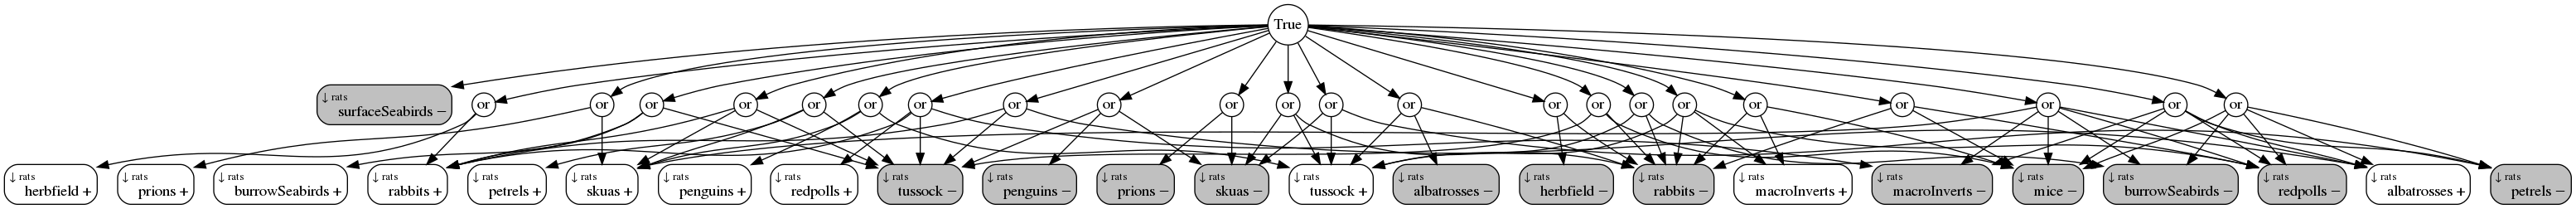
\includegraphics{attempt_1.png}

    To simplify a network, a good first step is to split the PCUs up by
length and present them in separate networks. Provided that every PCU is
represented in the networks, then no information will be lost.

It is also a good idea to put highly-connected responses, and other
pests, at the top as antecedents. We can spot highly-connected nodes by
the number of arrows that are feeding into them, and placing other pest
species at the top may be useful to decision-makers who are considering
either flow-on effects on other pests, or a multi-species control
programme.

    \begin{Verbatim}[commandchars=\\\{\}]
{\color{incolor}In [{\color{incolor}11}]:} \PY{n}{PCUList1} \PY{o}{=} \PY{p}{[} \PY{n}{PCU} \PY{k}{for} \PY{n}{PCU} \PY{o+ow}{in} \PY{n}{PCUList} \PY{k}{if} \PY{n+nb}{len}\PY{p}{(}\PY{n}{PCU}\PY{p}{)} \PY{o}{\PYZlt{}}\PY{o}{=} \PY{l+m+mi}{2} \PY{p}{]}
         \PY{n}{PCUList2} \PY{o}{=} \PY{p}{[} \PY{n}{PCU} \PY{k}{for} \PY{n}{PCU} \PY{o+ow}{in} \PY{n}{PCUList} \PY{k}{if} \PY{n+nb}{len}\PY{p}{(}\PY{n}{PCU}\PY{p}{)} \PY{o}{\PYZgt{}} \PY{l+m+mi}{2} \PY{p}{]}
         
         \PY{n}{draw\PYZus{}implication\PYZus{}network2}\PY{p}{(}\PY{n}{PCUList1}\PY{p}{,} 
             \PY{p}{[}\PY{p}{]}\PY{p}{,} 
             \PY{l+s+s1}{\PYZsq{}}\PY{l+s+s1}{PCUList1\PYZus{}1}\PY{l+s+s1}{\PYZsq{}}\PY{p}{,} \PY{n}{niceNames} \PY{o}{=} \PY{k+kc}{None}\PY{p}{,} \PY{n}{controlSymbol} \PY{o}{=} \PY{l+s+s1}{\PYZsq{}}\PY{l+s+s1}{downarrow}\PY{l+s+s1}{\PYZsq{}}\PY{p}{)}
         \PY{n}{draw\PYZus{}implication\PYZus{}network2}\PY{p}{(}\PY{n}{PCUList2}\PY{p}{,} 
             \PY{p}{[}\PY{l+s+s1}{\PYZsq{}}\PY{l+s+s1}{negrats\PYZus{}rabbits}\PY{l+s+s1}{\PYZsq{}}\PY{p}{,} \PY{l+s+s1}{\PYZsq{}}\PY{l+s+s1}{posrats\PYZus{}rabbits}\PY{l+s+s1}{\PYZsq{}}\PY{p}{,} \PY{l+s+s1}{\PYZsq{}}\PY{l+s+s1}{posrats\PYZus{}tussock}\PY{l+s+s1}{\PYZsq{}}\PY{p}{,} \PY{l+s+s1}{\PYZsq{}}\PY{l+s+s1}{negrats\PYZus{}tussock}\PY{l+s+s1}{\PYZsq{}}\PY{p}{]}\PY{p}{,}
             \PY{l+s+s1}{\PYZsq{}}\PY{l+s+s1}{PCUList2\PYZus{}1}\PY{l+s+s1}{\PYZsq{}}\PY{p}{,} \PY{n}{niceNames} \PY{o}{=} \PY{k+kc}{None}\PY{p}{,} \PY{n}{controlSymbol} \PY{o}{=} \PY{l+s+s1}{\PYZsq{}}\PY{l+s+s1}{downarrow}\PY{l+s+s1}{\PYZsq{}}\PY{p}{)}
         
         \PY{n}{os}\PY{o}{.}\PY{n}{system}\PY{p}{(}\PY{l+s+s2}{\PYZdq{}}\PY{l+s+s2}{dot \PYZhy{}Tpng PCUList1\PYZus{}1.dot \PYZgt{} PCUList1\PYZus{}1.png}\PY{l+s+s2}{\PYZdq{}}\PY{p}{)}
         \PY{n}{os}\PY{o}{.}\PY{n}{system}\PY{p}{(}\PY{l+s+s2}{\PYZdq{}}\PY{l+s+s2}{dot \PYZhy{}Tpng PCUList2\PYZus{}1.dot \PYZgt{} PCUList2\PYZus{}1.png}\PY{l+s+s2}{\PYZdq{}}\PY{p}{)}
\end{Verbatim}


    \begin{Verbatim}[commandchars=\\\{\}]
PCUList1\_1.pdf has been created
PCUList2\_1.pdf has been created

    \end{Verbatim}

\begin{Verbatim}[commandchars=\\\{\}]
{\color{outcolor}Out[{\color{outcolor}11}]:} 0
\end{Verbatim}
            
    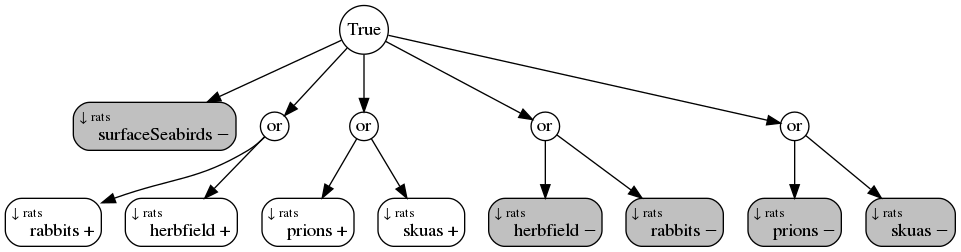
\includegraphics{PCUList1_1.png} \texttt{PCUList1\_1}

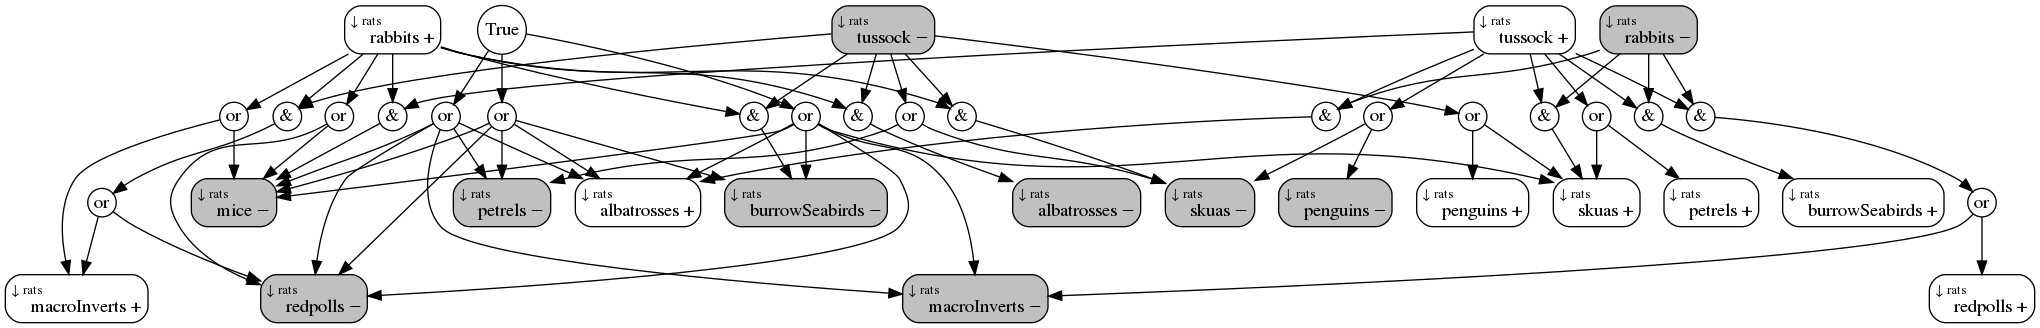
\includegraphics{PCUList2_1.png} \texttt{PCUList2\_1}

    In the top network (\texttt{PCUList1}), we recognise the same
bidirectional implication relationship that appeared previously, in the
network representing rabbit control. Rabbits and herbfield are also in a
bidirectional relationship. For short implications, the function
\texttt{draw\_implication\_network} can be more useful. It will repeat
the information contained in some of the PCUs (e.g. showing both
bidirectional outcomes), but when the implications are short, this
doesn't increase the complexity of the network much compared to the
increase in clarity of the implications' meaning.

    \begin{Verbatim}[commandchars=\\\{\}]
{\color{incolor}In [{\color{incolor}5}]:} \PY{n}{draw\PYZus{}implication\PYZus{}network}\PY{p}{(}\PY{n}{PCUList1}\PY{p}{,} 
                                 \PY{l+s+s1}{\PYZsq{}}\PY{l+s+s1}{PCUList1\PYZus{}2}\PY{l+s+s1}{\PYZsq{}}\PY{p}{,} 
                                 \PY{n}{niceNames} \PY{o}{=} \PY{k+kc}{None}\PY{p}{,} 
                                 \PY{n}{controlSymbol} \PY{o}{=} \PY{l+s+s1}{\PYZsq{}}\PY{l+s+s1}{downarrow}\PY{l+s+s1}{\PYZsq{}}\PY{p}{)}
        \PY{n}{os}\PY{o}{.}\PY{n}{system}\PY{p}{(}\PY{l+s+s2}{\PYZdq{}}\PY{l+s+s2}{dot \PYZhy{}Tpng PCUList1\PYZus{}2.dot \PYZgt{} PCUList1\PYZus{}2.png}\PY{l+s+s2}{\PYZdq{}}\PY{p}{)}
\end{Verbatim}


    \begin{Verbatim}[commandchars=\\\{\}]
PCUList1\_2.pdf has been created

    \end{Verbatim}

\begin{Verbatim}[commandchars=\\\{\}]
{\color{outcolor}Out[{\color{outcolor}5}]:} 0
\end{Verbatim}
            
    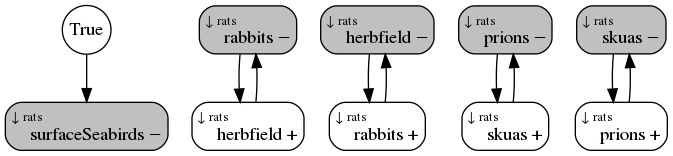
\includegraphics{PCUList1_2.png} \texttt{PCUList1\_2}

    In the second network (\texttt{PCUList2}), we see that a symmetry in the
effect of the combined response in rabbits and tussock. We can split
those out into two separate networks and place the remainder of the PCUs
in \texttt{PCUList5} for further analysis.

    \begin{Verbatim}[commandchars=\\\{\}]
{\color{incolor}In [{\color{incolor}6}]:} \PY{n}{PCUList3} \PY{o}{=} \PY{n+nb}{list}\PY{p}{(}\PY{p}{)} \PY{c+c1}{\PYZsh{} rat and tussock relationships}
        \PY{n}{PCUList4} \PY{o}{=} \PY{n+nb}{list}\PY{p}{(}\PY{p}{)}
        \PY{n}{PCUList5} \PY{o}{=} \PY{n+nb}{list}\PY{p}{(}\PY{p}{)} \PY{c+c1}{\PYZsh{} other}
        \PY{k}{for} \PY{n}{PCU} \PY{o+ow}{in} \PY{n}{PCUList2}\PY{p}{:}
            
            \PY{k}{if} \PY{l+s+s1}{\PYZsq{}}\PY{l+s+s1}{posrats\PYZus{}rabbits}\PY{l+s+s1}{\PYZsq{}} \PY{o+ow}{in} \PY{n}{PCU} \PY{o+ow}{and} \PY{l+s+s1}{\PYZsq{}}\PY{l+s+s1}{negrats\PYZus{}tussock}\PY{l+s+s1}{\PYZsq{}} \PY{o+ow}{in} \PY{n}{PCU}\PY{p}{:}
                \PY{n}{PCUList3}\PY{o}{.}\PY{n}{append}\PY{p}{(}\PY{n}{PCU}\PY{p}{)}
            \PY{k}{elif} \PY{l+s+s1}{\PYZsq{}}\PY{l+s+s1}{negrats\PYZus{}rabbits}\PY{l+s+s1}{\PYZsq{}} \PY{o+ow}{in} \PY{n}{PCU} \PY{o+ow}{and} \PY{l+s+s1}{\PYZsq{}}\PY{l+s+s1}{posrats\PYZus{}tussock}\PY{l+s+s1}{\PYZsq{}} \PY{o+ow}{in} \PY{n}{PCU}\PY{p}{:}
                \PY{n}{PCUList4}\PY{o}{.}\PY{n}{append}\PY{p}{(}\PY{n}{PCU}\PY{p}{)}
            \PY{k}{else}\PY{p}{:}
                \PY{n}{PCUList5}\PY{o}{.}\PY{n}{append}\PY{p}{(}\PY{n}{PCU}\PY{p}{)}
        
        \PY{n}{draw\PYZus{}implication\PYZus{}network2}\PY{p}{(}\PY{n}{PCUList3}\PY{p}{,} 
                    \PY{p}{[}\PY{l+s+s1}{\PYZsq{}}\PY{l+s+s1}{posrats\PYZus{}rabbits}\PY{l+s+s1}{\PYZsq{}}\PY{p}{,} \PY{l+s+s1}{\PYZsq{}}\PY{l+s+s1}{negrats\PYZus{}tussock}\PY{l+s+s1}{\PYZsq{}}\PY{p}{]}\PY{p}{,}
                    \PY{l+s+s1}{\PYZsq{}}\PY{l+s+s1}{PCUList3\PYZus{}1}\PY{l+s+s1}{\PYZsq{}}\PY{p}{,} \PY{n}{niceNames} \PY{o}{=} \PY{k+kc}{None}\PY{p}{,} \PY{n}{controlSymbol} \PY{o}{=} \PY{l+s+s1}{\PYZsq{}}\PY{l+s+s1}{downarrow}\PY{l+s+s1}{\PYZsq{}}\PY{p}{)}
        \PY{n}{draw\PYZus{}implication\PYZus{}network2}\PY{p}{(}\PY{n}{PCUList4}\PY{p}{,} 
                    \PY{p}{[}\PY{l+s+s1}{\PYZsq{}}\PY{l+s+s1}{negrats\PYZus{}rabbits}\PY{l+s+s1}{\PYZsq{}}\PY{p}{,} \PY{l+s+s1}{\PYZsq{}}\PY{l+s+s1}{posrats\PYZus{}tussock}\PY{l+s+s1}{\PYZsq{}}\PY{p}{]}\PY{p}{,}
                    \PY{l+s+s1}{\PYZsq{}}\PY{l+s+s1}{PCUList4\PYZus{}1}\PY{l+s+s1}{\PYZsq{}}\PY{p}{,} \PY{n}{niceNames} \PY{o}{=} \PY{k+kc}{None}\PY{p}{,} \PY{n}{controlSymbol} \PY{o}{=} \PY{l+s+s1}{\PYZsq{}}\PY{l+s+s1}{downarrow}\PY{l+s+s1}{\PYZsq{}}\PY{p}{)}
        
        \PY{n}{os}\PY{o}{.}\PY{n}{system}\PY{p}{(}\PY{l+s+s2}{\PYZdq{}}\PY{l+s+s2}{dot \PYZhy{}Tpng PCUList3\PYZus{}1.dot \PYZgt{} PCUList3\PYZus{}1.png}\PY{l+s+s2}{\PYZdq{}}\PY{p}{)}
        \PY{n}{os}\PY{o}{.}\PY{n}{system}\PY{p}{(}\PY{l+s+s2}{\PYZdq{}}\PY{l+s+s2}{dot \PYZhy{}Tpng PCUList4\PYZus{}1.dot \PYZgt{} PCUList4\PYZus{}1.png}\PY{l+s+s2}{\PYZdq{}}\PY{p}{)}
                    
\end{Verbatim}


    \begin{Verbatim}[commandchars=\\\{\}]
PCUList3\_1.pdf has been created
PCUList4\_1.pdf has been created

    \end{Verbatim}

\begin{Verbatim}[commandchars=\\\{\}]
{\color{outcolor}Out[{\color{outcolor}6}]:} 0
\end{Verbatim}
            
    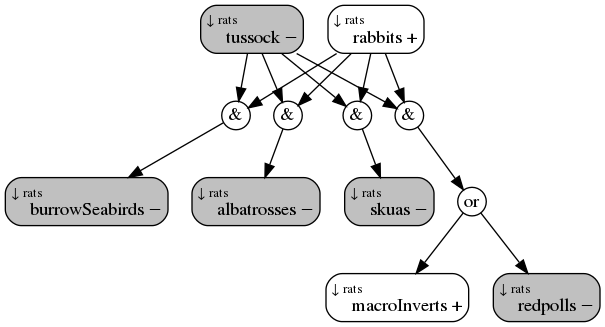
\includegraphics{PCUList3_1.png} \texttt{PCUList3\_1}

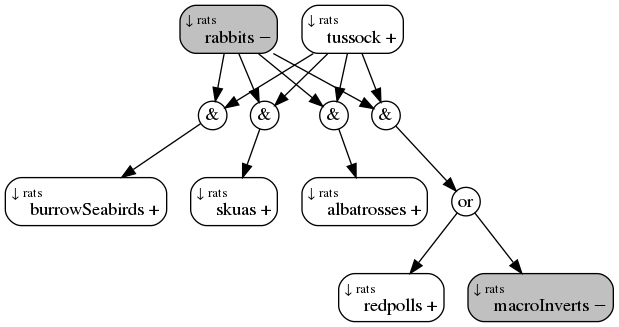
\includegraphics{PCUList4_1.png} \texttt{PCUList4\_1}

    The symmetry between the two scenarios above may be useful for
understanding the whole-system behaviour. For example, the response of
burrow-nesting seabirds and albatrosses echoes what was found for rabbit
control.

We now take a closer look at the PCUs that remain.

    \begin{Verbatim}[commandchars=\\\{\}]
{\color{incolor}In [{\color{incolor}7}]:} \PY{n}{draw\PYZus{}implication\PYZus{}network2}\PY{p}{(}\PY{n}{PCUList5}\PY{p}{,} 
                    \PY{p}{[}\PY{l+s+s1}{\PYZsq{}}\PY{l+s+s1}{posrats\PYZus{}mice}\PY{l+s+s1}{\PYZsq{}}\PY{p}{]}\PY{p}{,}
                    \PY{l+s+s1}{\PYZsq{}}\PY{l+s+s1}{PCUList5\PYZus{}1}\PY{l+s+s1}{\PYZsq{}}\PY{p}{,} \PY{n}{niceNames} \PY{o}{=} \PY{k+kc}{None}\PY{p}{,} \PY{n}{controlSymbol} \PY{o}{=} \PY{l+s+s1}{\PYZsq{}}\PY{l+s+s1}{downarrow}\PY{l+s+s1}{\PYZsq{}}\PY{p}{)}
        \PY{n}{os}\PY{o}{.}\PY{n}{system}\PY{p}{(}\PY{l+s+s2}{\PYZdq{}}\PY{l+s+s2}{dot \PYZhy{}Tpng PCUList5\PYZus{}1.dot \PYZgt{} PCUList5\PYZus{}1.png}\PY{l+s+s2}{\PYZdq{}}\PY{p}{)}
\end{Verbatim}


    \begin{Verbatim}[commandchars=\\\{\}]
PCUList5\_1.pdf has been created

    \end{Verbatim}

\begin{Verbatim}[commandchars=\\\{\}]
{\color{outcolor}Out[{\color{outcolor}7}]:} 0
\end{Verbatim}
            
    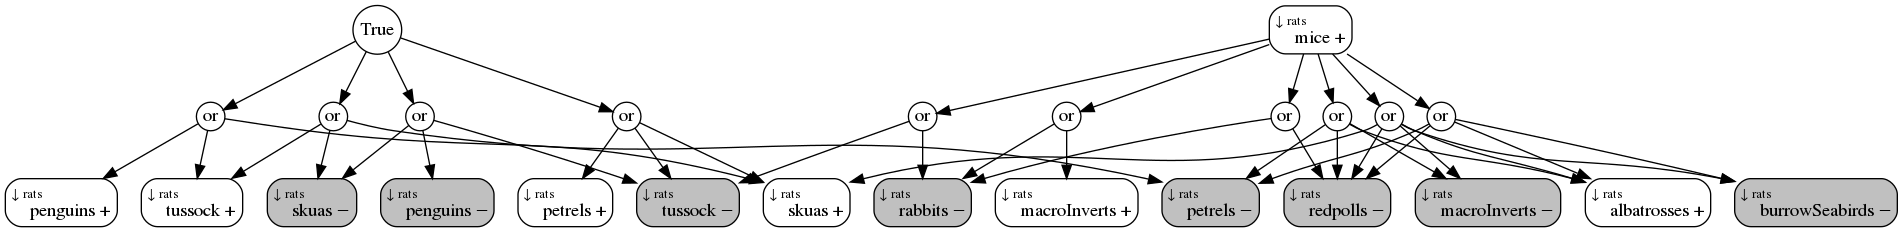
\includegraphics{PCUList5_1.png} \texttt{PCUList5\_1}

    There is an obvious split between relationships involving mice and not.
The relationships not involving mice have a symmetry, so we should
choose an arrangement that emphasises that. Below, we choose to place
the effect of rat control on tussock as the antecedent.

    \begin{Verbatim}[commandchars=\\\{\}]
{\color{incolor}In [{\color{incolor}8}]:} \PY{n}{PCUList6} \PY{o}{=} \PY{n+nb}{list}\PY{p}{(}\PY{p}{)} \PY{c+c1}{\PYZsh{} for rules without mice}
        \PY{n}{PCUList7} \PY{o}{=} \PY{n+nb}{list}\PY{p}{(}\PY{p}{)} \PY{c+c1}{\PYZsh{} for rules with mice}
        
        \PY{k}{for} \PY{n}{PCU} \PY{o+ow}{in} \PY{n}{PCUList5}\PY{p}{:}
            \PY{k}{if} \PY{l+s+s1}{\PYZsq{}}\PY{l+s+s1}{posrats\PYZus{}mice}\PY{l+s+s1}{\PYZsq{}} \PY{o+ow}{in} \PY{n}{PCU}\PY{p}{:}
                \PY{n}{PCUList7}\PY{o}{.}\PY{n}{append}\PY{p}{(}\PY{n}{PCU}\PY{p}{)}
            \PY{k}{else}\PY{p}{:}
                \PY{n}{PCUList6}\PY{o}{.}\PY{n}{append}\PY{p}{(}\PY{n}{PCU}\PY{p}{)}
        
        \PY{n}{draw\PYZus{}implication\PYZus{}network2}\PY{p}{(}\PY{n}{PCUList6}\PY{p}{,} 
                    \PY{p}{[}\PY{l+s+s1}{\PYZsq{}}\PY{l+s+s1}{posrats\PYZus{}tussock}\PY{l+s+s1}{\PYZsq{}}\PY{p}{,} \PY{l+s+s1}{\PYZsq{}}\PY{l+s+s1}{negrats\PYZus{}tussock}\PY{l+s+s1}{\PYZsq{}}\PY{p}{]}\PY{p}{,}
                    \PY{l+s+s1}{\PYZsq{}}\PY{l+s+s1}{PCUList6\PYZus{}1}\PY{l+s+s1}{\PYZsq{}}\PY{p}{,} \PY{n}{niceNames} \PY{o}{=} \PY{k+kc}{None}\PY{p}{,} \PY{n}{controlSymbol} \PY{o}{=} \PY{l+s+s1}{\PYZsq{}}\PY{l+s+s1}{downarrow}\PY{l+s+s1}{\PYZsq{}}\PY{p}{)}
        \PY{n}{os}\PY{o}{.}\PY{n}{system}\PY{p}{(}\PY{l+s+s2}{\PYZdq{}}\PY{l+s+s2}{dot \PYZhy{}Tpng PCUList6\PYZus{}1.dot \PYZgt{} PCUList6\PYZus{}1.png}\PY{l+s+s2}{\PYZdq{}}\PY{p}{)}
\end{Verbatim}


    \begin{Verbatim}[commandchars=\\\{\}]
PCUList6\_1.pdf has been created

    \end{Verbatim}

\begin{Verbatim}[commandchars=\\\{\}]
{\color{outcolor}Out[{\color{outcolor}8}]:} 0
\end{Verbatim}
            
    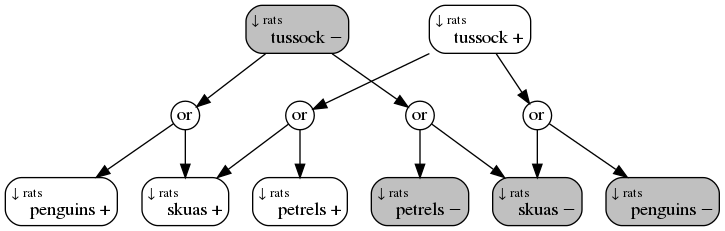
\includegraphics{PCUList6_1.png} \texttt{PCUList6\_1}

    Now we consider the right-hand side, the relationships involving mice.

The importance of tussock suggests that the interaction between rabbits,
mice, and tussock may be interesting in its own right. The simultaneous
effect on rabbits is also involved in outcomes for macroinvertebrates
and redpolls, and rabbits are another pest species, so we move the
rabbit response to the antecedent.

    \begin{Verbatim}[commandchars=\\\{\}]
{\color{incolor}In [{\color{incolor}9}]:} \PY{n}{draw\PYZus{}implication\PYZus{}network2}\PY{p}{(}\PY{n}{PCUList7}\PY{p}{,} 
                    \PY{p}{[}\PY{l+s+s1}{\PYZsq{}}\PY{l+s+s1}{posrats\PYZus{}rabbits}\PY{l+s+s1}{\PYZsq{}}\PY{p}{,} \PY{l+s+s1}{\PYZsq{}}\PY{l+s+s1}{posrats\PYZus{}mice}\PY{l+s+s1}{\PYZsq{}}\PY{p}{]}\PY{p}{,}
                    \PY{l+s+s1}{\PYZsq{}}\PY{l+s+s1}{PCUList7\PYZus{}1}\PY{l+s+s1}{\PYZsq{}}\PY{p}{,} \PY{n}{niceNames} \PY{o}{=} \PY{k+kc}{None}\PY{p}{,} \PY{n}{controlSymbol} \PY{o}{=} \PY{l+s+s1}{\PYZsq{}}\PY{l+s+s1}{downarrow}\PY{l+s+s1}{\PYZsq{}}\PY{p}{)}
        \PY{n}{os}\PY{o}{.}\PY{n}{system}\PY{p}{(}\PY{l+s+s2}{\PYZdq{}}\PY{l+s+s2}{dot \PYZhy{}Tpng PCUList7\PYZus{}1.dot \PYZgt{} PCUList7\PYZus{}1.png}\PY{l+s+s2}{\PYZdq{}}\PY{p}{)}
\end{Verbatim}


    \begin{Verbatim}[commandchars=\\\{\}]
PCUList7\_1.pdf has been created

    \end{Verbatim}

\begin{Verbatim}[commandchars=\\\{\}]
{\color{outcolor}Out[{\color{outcolor}9}]:} 0
\end{Verbatim}
            
    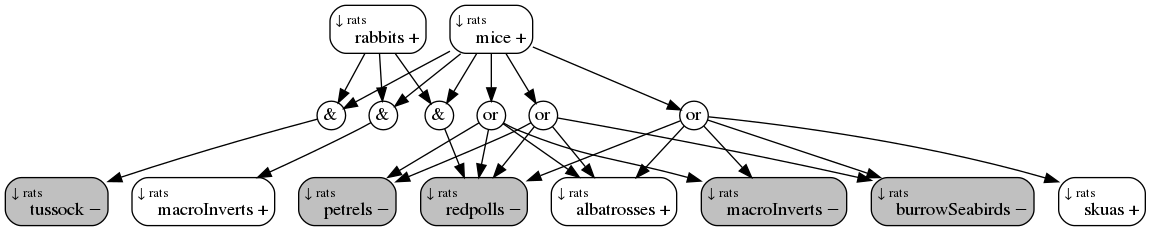
\includegraphics{PCUList7_1.png} \texttt{PCUList7\_1}

    One could end the splitting of the remaining PCUs here. Alternatively,
one could choose to emphasise the contingency upon the response of
redpolls, by further splitting the network.

    \begin{Verbatim}[commandchars=\\\{\}]
{\color{incolor}In [{\color{incolor}10}]:} \PY{n}{PCUList8} \PY{o}{=} \PY{n+nb}{list}\PY{p}{(}\PY{p}{)} \PY{c+c1}{\PYZsh{} for rabbit and mice relationships}
         \PY{n}{PCUList9} \PY{o}{=} \PY{n+nb}{list}\PY{p}{(}\PY{p}{)} \PY{c+c1}{\PYZsh{} the remainder, which all involve redpolls}
         
         \PY{k}{for} \PY{n}{PCU} \PY{o+ow}{in} \PY{n}{PCUList7}\PY{p}{:}
             \PY{k}{if} \PY{l+s+s1}{\PYZsq{}}\PY{l+s+s1}{posrats\PYZus{}rabbits}\PY{l+s+s1}{\PYZsq{}} \PY{o+ow}{in} \PY{n}{PCU}\PY{p}{:}
                 \PY{n}{PCUList8}\PY{o}{.}\PY{n}{append}\PY{p}{(}\PY{n}{PCU}\PY{p}{)}
             \PY{k}{else}\PY{p}{:}
                 \PY{n}{PCUList9}\PY{o}{.}\PY{n}{append}\PY{p}{(}\PY{n}{PCU}\PY{p}{)}
                 
         \PY{n}{draw\PYZus{}implication\PYZus{}network2}\PY{p}{(}\PY{n}{PCUList8}\PY{p}{,} 
                     \PY{p}{[}\PY{l+s+s1}{\PYZsq{}}\PY{l+s+s1}{posrats\PYZus{}rabbits}\PY{l+s+s1}{\PYZsq{}}\PY{p}{,} \PY{l+s+s1}{\PYZsq{}}\PY{l+s+s1}{posrats\PYZus{}mice}\PY{l+s+s1}{\PYZsq{}}\PY{p}{]}\PY{p}{,}
                     \PY{l+s+s1}{\PYZsq{}}\PY{l+s+s1}{PCUList8\PYZus{}1}\PY{l+s+s1}{\PYZsq{}}\PY{p}{,} \PY{n}{niceNames} \PY{o}{=} \PY{k+kc}{None}\PY{p}{,} \PY{n}{controlSymbol} \PY{o}{=} \PY{l+s+s1}{\PYZsq{}}\PY{l+s+s1}{downarrow}\PY{l+s+s1}{\PYZsq{}}\PY{p}{)}
         \PY{n}{os}\PY{o}{.}\PY{n}{system}\PY{p}{(}\PY{l+s+s2}{\PYZdq{}}\PY{l+s+s2}{dot \PYZhy{}Tpng PCUList8\PYZus{}1.dot \PYZgt{} PCUList8\PYZus{}1.png}\PY{l+s+s2}{\PYZdq{}}\PY{p}{)}
         
         \PY{n}{draw\PYZus{}implication\PYZus{}network2}\PY{p}{(}\PY{n}{PCUList9}\PY{p}{,} 
                     \PY{p}{[}\PY{l+s+s1}{\PYZsq{}}\PY{l+s+s1}{posrats\PYZus{}redpolls}\PY{l+s+s1}{\PYZsq{}}\PY{p}{,} \PY{l+s+s1}{\PYZsq{}}\PY{l+s+s1}{posrats\PYZus{}mice}\PY{l+s+s1}{\PYZsq{}}\PY{p}{]}\PY{p}{,}
                     \PY{l+s+s1}{\PYZsq{}}\PY{l+s+s1}{PCUList9\PYZus{}1}\PY{l+s+s1}{\PYZsq{}}\PY{p}{,} \PY{n}{niceNames} \PY{o}{=} \PY{k+kc}{None}\PY{p}{,} \PY{n}{controlSymbol} \PY{o}{=} \PY{l+s+s1}{\PYZsq{}}\PY{l+s+s1}{downarrow}\PY{l+s+s1}{\PYZsq{}}\PY{p}{)}
         \PY{n}{os}\PY{o}{.}\PY{n}{system}\PY{p}{(}\PY{l+s+s2}{\PYZdq{}}\PY{l+s+s2}{dot \PYZhy{}Tpng PCUList9\PYZus{}1.dot \PYZgt{} PCUList9\PYZus{}1.png}\PY{l+s+s2}{\PYZdq{}}\PY{p}{)}
\end{Verbatim}


    \begin{Verbatim}[commandchars=\\\{\}]
PCUList8\_1.pdf has been created
PCUList9\_1.pdf has been created

    \end{Verbatim}

\begin{Verbatim}[commandchars=\\\{\}]
{\color{outcolor}Out[{\color{outcolor}10}]:} 0
\end{Verbatim}
            
    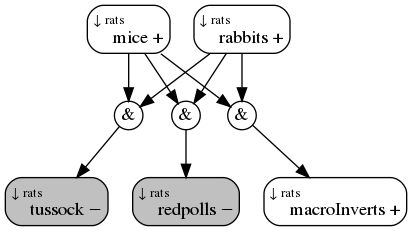
\includegraphics{PCUList8_1.png} \texttt{PCUList8\_1}

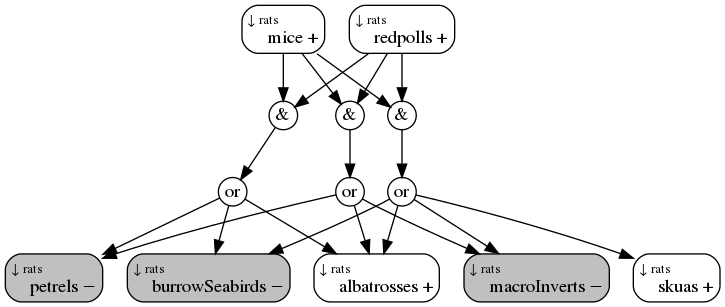
\includegraphics{PCUList9_1.png} \texttt{PCUList9\_1}

    \subsection{Potential final
presentation}\label{potential-final-presentation}

The presentation below combines all of the subnetworks that we split
above. The decisions that were made to produce this network were
somewhat arbitrary, and the best choice depends upon the needs of
conservation decision-makers, and may also reflect our causal
understanding of the relationships between species.

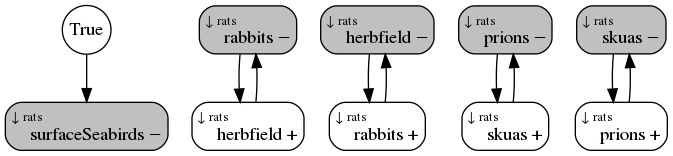
\includegraphics{PCUList1_2.png} 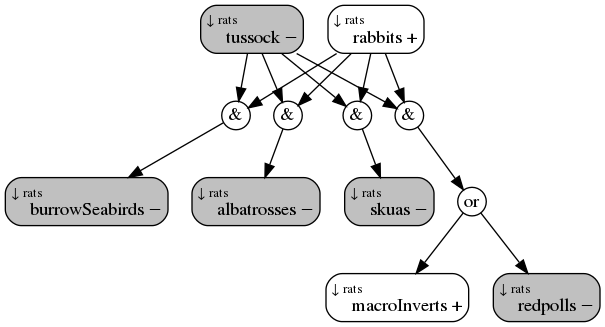
\includegraphics{PCUList3_1.png}
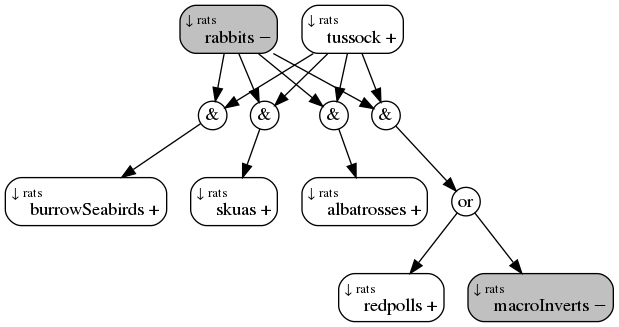
\includegraphics{PCUList4_1.png} 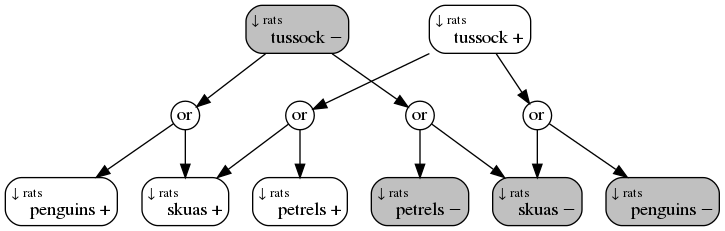
\includegraphics{PCUList6_1.png}
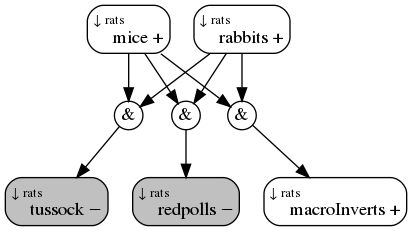
\includegraphics{PCUList8_1.png} 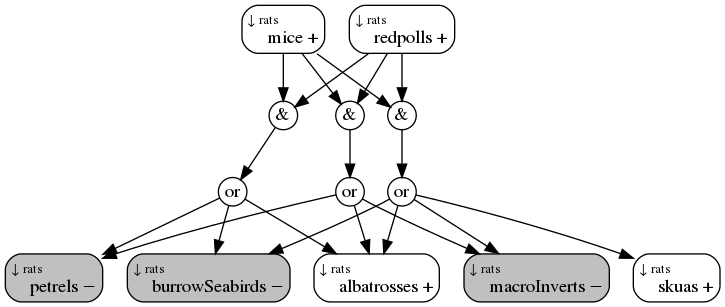
\includegraphics{PCUList9_1.png}


    % Add a bibliography block to the postdoc
    
    
    
    \end{document}
